\documentclass{article}

\usepackage[margin=1in]{geometry}
\usepackage{amsmath,amsthm,amssymb}
\usepackage{bbm, enumerate, tikz}
\usepackage{multicol}

\newenvironment{problem}[2][Problem]{\begin{trivlist}
\item[\hskip \labelsep {\bfseries #1}\hskip \labelsep {\bfseries #2.}]}{\end{trivlist}}
\newenvironment{note}[1][Note.]{\begin{trivlist}
\item[\hskip \labelsep {\bfseries #1}]}{\end{trivlist}}

\begin{document}

\title{Fall 2012: Complex Analysis Graduate Exam}
\author{Peter Kagey}

\maketitle

% -----------------------------------------------------
% First problem
% -----------------------------------------------------
\begin{problem}{1}
  Evaluate the integral \[
    \int_0^\infty \frac{dx}{1 + x^n}\,dx
  \] being careful to justify your methods.
\end{problem}

\begin{proof} $ $\\
  First notice that the integrand $f(z) = (1 + x^n)^{-1}$ has poles at \begin{align*}
    1 + x^n &= 0 \\
    x^n     &= e^{\pi i + 2\pi i k} \\
    z_k     &= e^{(2k + 1)\pi i/n} \text{ where } 0 \leq k < n.
  \end{align*}
  The idea is to draw a contour around the first pole $z_0 = e^{\pi i/n}$ along an $n$-th root
  of unity, and then compute the integral via the Residue Theorem.
  In particular, we will use the contour given by:
  \begin{multicols}{2}
  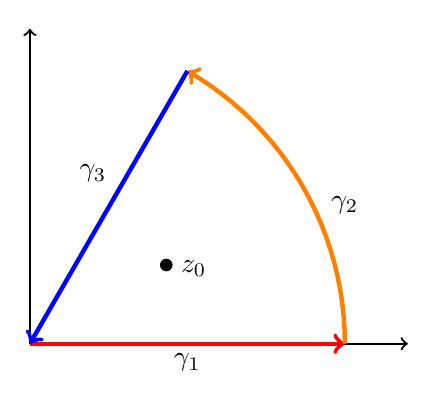
\begin{tikzpicture}[scale=0.8]
    % \draw[very thin,color=gray] (-0.9,-0.9) grid (5.9,5.9);
    \draw[thick, ->] (0,0)--(6,0);
    \draw[thick, ->] (0,0)--(0,5);
    \draw[ultra thick, ->, draw=red, domain=0:5] plot ({\x}, {0});
    \draw node at (2.5, -0.3) {$\gamma_{1}$};
    \draw[ultra thick, ->, draw=orange, domain=0:60] plot ({5*cos(\x)}, {5*sin(\x)});
    \draw node at (5, 2.2) {$\gamma_{2}$};
    \draw[ultra thick, <-, draw=blue, domain=0:5] plot ({\x*cos(60)}, {\x*sin(60)});
    \draw node at (1, 2.7) {$\gamma_{3}$};
    \fill ({2.5*cos(30)}, {2.5 * sin(30)}) circle (0.1);
    \draw node at (2.6, 1.2) {$z_0$};
  \end{tikzpicture}\\
  \begin{align}
    \gamma_{1} &= \{t + 0i\ |\ x \in [0, R] \} \\
    \gamma_{2} &= \{R e^{it}\ |\ t \in [0,2\pi/n] \} \\
    \gamma_{3} &= \{t e^{2\pi i/n}\ |\ t \in [0, R]\}
  \end{align}
  \end{multicols}
  \[
    \int_{\gamma_1} f(z)\,dz +
    \int_{\gamma_2} f(z)\,dz +
    \int_{\gamma_3} f(z)\,dz =
    2\pi i \operatorname{Res}_{z_0}(f).
  \]
  In the limit, the integral over $\gamma_2$ vanishes.
  \begin{align*}
    \left|\int_{\gamma_2}f(z)\,dz\right|
    &= \left|
      \int_0^{2\pi/n}\frac{dt}{1 + {(Re^{it})^n}}iRe^{it}
    \right|\\
    &\leq \int_0^{2\pi/n}\left|
      \frac{iRe^{it}}{1 + R^ne^{tni}}
    \right|\, dt \\
    &\leq \int_0^{2\pi/n}\left|
      \frac{iRe^{it}}{R^ne^{tni}}
    \right|\, dt \\
    &= \frac{1}{R^{n - 1}}\int_0^{2\pi/n}\,dt \\
    &= \frac{2\pi}{nR^{n - 1}}
  \end{align*} which vanishes as $R \rightarrow \infty$.
  This means that our equation simplifies in the limit to \[
    \int_{\gamma_1} f(z)\,dz +
    \int_{\gamma_3} f(z)\,dz =
    2\pi i \operatorname{Res}_{z_0}(f).
  \]
  Also the integral over $\gamma_3$ is a multiple of the integral over
  $\gamma_1$,
  \begin{align*}
    \int_R^0\frac{1}{1 + (te^{2\pi i/n})^n}e^{2\pi i/n}\,dt &=
    -e^{2\pi i/n}\int_0^R\frac{dt}{1 + t^n}\\
    &= -e^{2\pi i/n}\int_{\gamma_1} f(z)\,dz,
  \end{align*}
  so the equation further simplifies to \[
  \int_{\gamma_1} f(z)\,dz -
  e^{2\pi i/n} \int_{\gamma_1} f(z)\,dz =
  2\pi i \operatorname{Res}_{z_0}(f).
  \]
  So by the Residue Theorem, the integral evaluates to \[
    \int_{\gamma_1} f(z)\,dz = \frac{2\pi i \operatorname{Res}_{z_0}(f)}{1 - e^{2\pi i/n}},
  \] and it is enough to compute the residue: \[
    \operatorname{Res}_{z_0}(f)
    = \lim_{z \rightarrow z_0} (z - z_0) f(z)
    = \lim_{z \rightarrow z_0} \frac{1}{\displaystyle\left(
      \frac{1 + z^n}{z - z_0}
    \right)}
    = \frac{1}{\displaystyle\frac{d}{dz}\left[
      1 + z^n
    \right]_{z = z_0}}
    = \frac{1}{n z_0^{n-1}}
  \]
  Therefore \begin{align*}
    \int_0^\infty\frac{dx}{1 + x^n}
    &= \frac{2\pi i}{nz_0^{n-1}(1 - e^{2\pi i/n})} \\
    % &= \frac{2\pi i/n}{z_0^{n-1}(1 - e^{2\pi i/n})} \\
    &= \frac{2\pi i/n}{e^{\pi i(n-1)/n}(1 - e^{2\pi i/n})} \\
    &= \frac{2\pi i/n}{\underbrace{e^{\pi i}}_{=-1} e^{-\pi i/n}(1 - e^{2\pi i/n})} \\
    &= \frac{2\pi i/n}{-e^{-\pi i/n} + e^{\pi i/n}} \\
    &= \frac{\pi}{n}\cdot\displaystyle\left(
      \frac{e^{\pi i/n}-e^{-\pi i/n}}{2i}
    \right)^{-1} \\
    &= \frac{\pi}{n \sin(\pi/n)}
  \end{align*}
\end{proof}
% -----------------------------------------------------
% Second problem
% -----------------------------------------------------
\pagebreak

\begin{problem}{2}
  Find the Laurent series expansion for \[
    \frac{1}{z(z+1)}
  \] valid in $\{ 1 < |z - 1| < 2\}$.
\end{problem}

\begin{proof}
  It is easiest to find the expansion centered at $0$, so we will instead
  substitute $z - 1 = w$ and find the Laurent series expansion of \[
    \hat f(w) = \frac{1}{(w + 1)(w + 2)}
  \] valid when $1 < |w| < 2$.
  \\
  Notice that by partial fraction decomposition, \[
    \frac{1}{(w + 1)(w + 2)} = \frac{A}{w + 1} + \frac{B}{w + 2}
  \] where $A$ and $B$ satisfy the system of equations \begin{align*}
      A + B = 0 \\
      2A + B = 1
  \end{align*} and so $A = 1$ and $B = -1$.
  \\
  Now we can add the Laurent series expansion of the two summands to give the
  Laurent series of $\hat f$.
  \\~\\
  \textbf{Laurent series of $(w+1)^{-1}$ for $|w| > 1$.}\\
  Notice that \[
    \frac{1}{w + 1} = \frac{1}{w}\cdot\frac{1}{1 - (-\frac{1}{w})}
    = \frac{1}{w}\sum_{n=0}^\infty\left(\frac{-1}{w}\right)^n
    = -\sum_{n=1}^\infty (-1)^{-n}w^{-n}
  \] for $|1/w| < 1$ (or equivalently $|w| > 1$).
  \\~\\
  \textbf{Laurent series of $-(w+2)^{-1}$ for $|w| < 2$.}\\
  Similarly \[
    \frac{1}{w + 2} = \frac{1}{2}\cdot\frac{1}{1 - (-\frac{w}{2})}
    = \frac{1}{2}\sum_{n=0}^\infty\left(\frac{-w}{2}\right)^n
    = -\sum_{n=0}^\infty \left(-\frac{1}{2}\right)^{n+1}w^n
  \] for $|w/2| < 1$ (or equivalently $|w| < 2$).
  \\~\\
  Thus the Laurent series of $\hat f$ is \[
    \hat f(w) = -\sum_{n=1}^\infty (-1)^{-n}w^{-n}
    -\sum_{n=0}^\infty \left(-\frac{1}{2}\right)^{n+1}w^n,
  \] in $\{ 1 < |w| < 2\}$, so the Laurent series of $f$ is \[
    f(z) = -\sum_{n=1}^\infty (-1)^{-n}(z - 1)^{-n}
    -\sum_{n=0}^\infty \left(-\frac{1}{2}\right)^{n+1}(z - 1)^n
  \] in $\{ 1 < |z - 1| < 2\}$.
\end{proof}

% -----------------------------------------------------
% Third problem
% -----------------------------------------------------
\pagebreak

\begin{problem}{3}
  Suppose that $f$ is an entire function and that there is a bounded sequence of
  distinct real numbers $a_1, a_2, a_3, \hdots$ such that $f(a_k)$ is real for
  each $k$. Show that $f(x)$ is real for all real $x$.
\end{problem}

\begin{proof}
  Because the sequence of real numbers is bounded, there must be a (real)
  accumulation point by the Bolzano-Weierstrass Theorem; call it $z_0$.
  \\~\\
  Now, since $f$ is entire, we can do a Taylor Series expansion about $z_0$.
  All derivatives are real, because we can always find real $z$ arbitrarily
  close to $z_0$ and both the numerator and denominator in the definition of the
  derivative are real, \[
    \lim_{z \rightarrow z_0} \frac{f(z) - f(z_0)}{z - z_0},
  \] so the derivative itself is real.
  \\
  This same idea works for higher order derivatives, so the Taylor expansion
  about $z_0$ has all real coefficients. Therefore, $f(x)$ is real-valued for
  all real $x$.
\end{proof}

% -----------------------------------------------------
% Fourth problem
% -----------------------------------------------------
\pagebreak

\begin{problem}{4}
  Suppose \[
    f_n(z) = \sum_{k=0}^n\frac{1}{k!z^k},\ z \neq 0
  \] and let $\varepsilon > 0$. Show that for large enough $n$ all the zeros of
  $f_n$ are in the disk $D(0, \varepsilon)$ with center 0 and radius $\varepsilon$
\end{problem}

\begin{proof}
  % It would be nice to use Rouch\'e's Theorem directly, but we can't since $f_n$
  % is not analytic on $D(0, \varepsilon)$. So instead we will consider the
  % polynomials $\hat f_n(z) = f_n(1/z)$ and show that for sufficiently large $n$,
  % these have zero roots inside of $1/\varepsilon$.
  % \\~\\
  The plan here is to show that the function $\hat f_n(x) = f_n(1/x)$ has no
  zeros inside the disk of radius $R = 1/\varepsilon$ for any large $R$ and
  sufficiently large $n$.

  Since $\hat f_n(z)$ is just a partial sum of the Taylor series of $e^z$, which
  converges
\end{proof}

\end{document}
